
\documentclass[twoside,a4paper]{article}

\usepackage{blindtext} % Package to generate dummy text throughout this template 

\usepackage[sc]{mathpazo} % Use the Palatino font
\usepackage[T1]{fontenc} % Use 8-bit encoding that has 256 glyphs
\linespread{1.05} % Line spacing - Palatino needs more space between lines
\usepackage{microtype} % Slightly tweak font spacing for aesthetics

%\usepackage[english]{babel}
\usepackage[none]{hyphenat} % Disable hyphenation for now

\usepackage[document]{ragged2e} % Disable text justification

\usepackage[left=1cm,right=1cm,hmarginratio=1:1,top=2cm,bottom=2cm,columnsep=20pt]{geometry} % Document margins
\usepackage[hang, small,labelfont=bf,up,textfont=it,up]{caption} % Custom captions under/above floats in tables or figures
\usepackage{booktabs} % Horizontal rules in tables
\usepackage{nameref} % Named references
\usepackage{enumitem} % Customized lists

\setlist[itemize]{noitemsep} % Make itemize lists more compact
\usepackage{tikz}

\usepackage{titlesec} % Allows customization of titles
\titleformat{\section}{\large\scshape}{\thesection.\index{}}{1em}{} % Change the look of the section titles
\titleformat{\subsection}{\large}{\thesubsection.\index{}}{1em}{} % Change the look of the section titles
\titleformat{\subsubsection}{\large}{\thesubsection.\index{}}{1em}{} % Change the look of the section titles
\usepackage{sectsty}% http://ctan.org/pkg/sectsty
\usepackage{titlecaps}% http://ctan.org/pkg/titlecaps
\subsubsectionfont{\MakeUppercase}

\usepackage{titling} % Customizing the title section

\usepackage{ulem}
\usepackage{contour}

\renewcommand{\ULdepth}{1.8pt}
\contourlength{0.8pt}

\newcommand{\myuline}[1]{
\uline{\phantom{#1}}\llap{\contour{white}{#1}}%
}
\usepackage{scrextend}
\usepackage{imakeidx}
\makeindex[columns=3, title=Index, options= -s index_style.ist, intoc, columnsep=.5cm]
\usepackage[pdfborderstyle={/S/U/W 1},linktoc=all]{hyperref} % For hyperlinks in the PDF

\def\nf{1}
\newcommand{\related}[1]{
\def\relatedtopicslist{#1}
\textbf{Related topics:} \foreach \x [count=\xi] in \relatedtopicslist{\ifnum\xi>1, \fi\myuline{\nameref{\x} (\pageref{\x})}}
}

\newcommand*{\seeonpage}[1]{
\def\pagelabel{#1}
\hyperref[{\pagelabel}]{See \myuline{"\nameref*{\pagelabel}" on page \pageref*{\pagelabel}}}
}

\newcommand{\newreference}[2]{
	\subsubsection{#1}
	\label{#2}
	\index{#1}
}

%Fix very long index hanging issue
\makeatletter
\def\@idxitem{\par\hangindent 0pt}
\makeatother

\setlength{\parindent}{0em}
\setlength{\parskip}{1em}
\setlist[itemize]{noitemsep, topsep=0pt}
\twocolumn
\usepackage{fancyhdr}
\fancyhf{} % clear all header and footers
\pagestyle{fancy}
\rfoot{\thepage}

\makeatletter
\def\@seccntformat#1{%\fi\fi
  \expandafter\ifx\csname c@#1\endcsname\c@subsubsection\else
  \csname the#1\endcsname\quad
  \fi}
\makeatother

%%%%%%%%%%%%%%%%%%%%%%%%%%%%%%%%%%%%


\title{Dungeon Alliance Community Reference Rules Guide} % Article title
\begin{document}\sloppy

\newcommand{\documentversion}{v0.1}

%----------------------------------------------------------------------------------------
%	COVER PAGE
%----------------------------------------------------------------------------------------
\thispagestyle{empty}
\onecolumn
\newgeometry{left=0cm,bottom=0.15cm,right=0cm,top=0cm}

\backgroundsetup{
scale=1,
color=black,
angle=0,
opacity=1,
contents={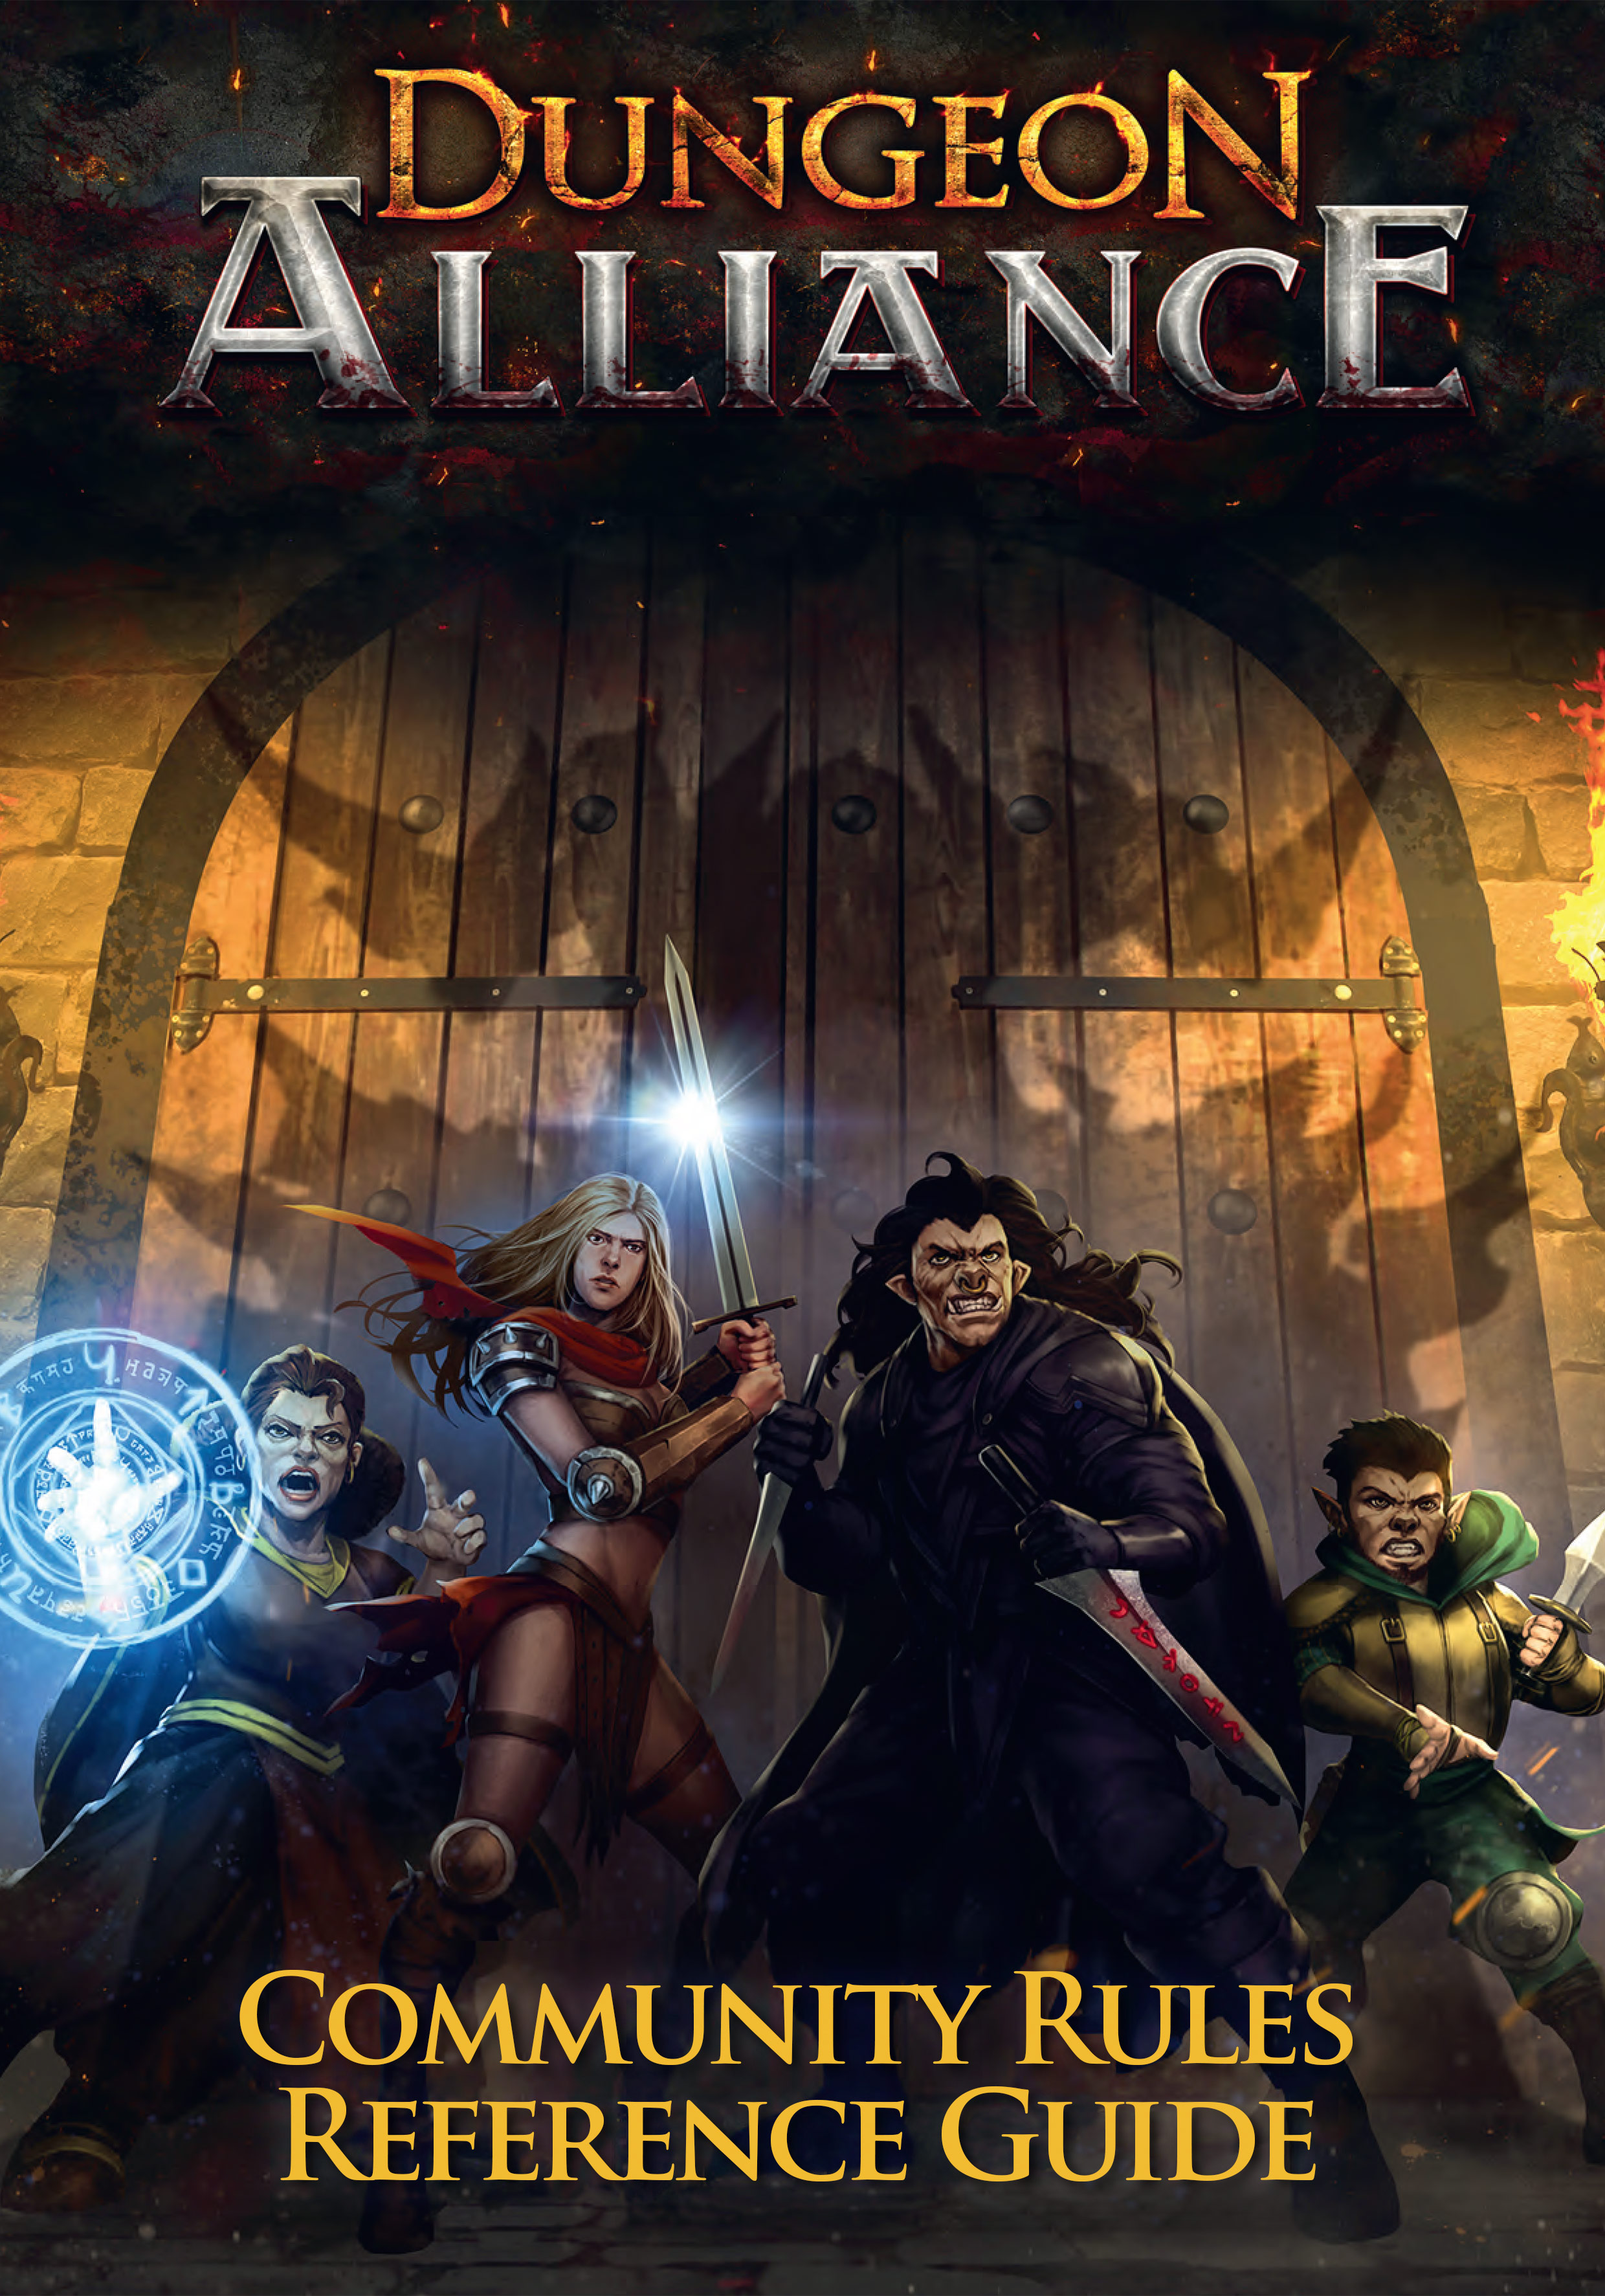
\includegraphics[width=\paperwidth,height=\paperheight]{images/cover.jpg}}
}

\vspace*{\fill}
\begin{center}
\color{versionnrcolor}\trajan\fontsize{16}{16}\selectfont
\documentversion
\end{center}
%
%----------------------------------------------------------------------------------------
%	PREFACE & CONTENTS
%----------------------------------------------------------------------------------------
\clearpage
\restoregeometry
\backgroundsetup{
scale=1,
color=black,
angle=90,
contents={%
 \checkoddpage
  \ifoddpage
   
\includegraphics[width=\paperheight,height=\paperwidth]{images/page_background.jpg}
  \else
   
\includegraphics[width=\paperheight,height=\paperwidth]{images/page_background.jpg}
  \fi
  }%
}

\section{Preface}
\label{sec:Preface}
This Community Rules Reference Guide (CRRG) is a comprehensive cross-reference and resource for all Dungeon Alliance rules. Unlike the rulebook and rules supplement from the base game, it addresses complex and unusual game-play situations.

This community reference covers the following areas:
\begin{itemize}
\item Rules from the base game including rules supplement and all released expansions
\item Visual examples for "Movement", "Line of Sight" and "Special
Situations in Combat"
\item Tables with overviews on the content of the base game and expansions
\item An index with hyperlinked page numbers
\end{itemize}

\textbf{Section \ref*{sec:RulesReferenceGuide}} lists the rules of the game in alphabetical order. It should allow players to quickly find answers to questions during gameplay by looking up the entry in question. Each entry includes the basic rules, with exceptions and additional clarifications. Related topics below each entry link to other entries that hold additional information.

\textbf{Section \ref*{sec:ErrataAndFAQ}} contains errata and frequently asked questions. Here you can find clarifications for example on how a certain card effect is meant to be played.

\textbf{Section \ref*{sec:Appendix}} contains different tables detailing for example the content of the game and it's expansions.

\noindent\hfil\rule{2cm}{.2pt}\hfil

\textbf{DISCLAIMER:} This document is currently very incomplete and should not be used as a reference for the game in it's current form.

\noindent\hfil\rule{2cm}{.2pt}\hfil

This CRRG is a fan-made guide and might not offer the same level of quality as the official rule books. Mistakes and typos are very probable. All feedback is wholeheartedly welcome!

This guide has been very much influenced by the excellent \myuline{\href{http://descent-community.org/index.php/crrg/}{Descent Community Rules Reference Guide}} available for Descent: Journeys in the Dark Second Edition and maintained by \textbf{Sadgit}.

\noindent\hfil\rule{2cm}{.2pt}\hfil

Quixotic Games LLC has generously given the permission to include text excerpts, images and artwork from the official rulebooks. This material is Copyright 2017 Quixotic Games LLC.

\newpage
\setcounter{secnumdepth}{4}
\setcounter{tocdepth}{2}
\tableofcontents

%----------------------------------------------------------------------------------------
%	RULES REFERENCE GUIDE
%----------------------------------------------------------------------------------------
\section{Rules Reference Guide}
\label{sec:RulesReferenceGuide}

\newreference{Ability bonus}{sec:Abilitybonus}
Many Starting Deck Cards and Upgrade Cards provide an Ability Bonus ( TBD see image), which is considered to be in effect for the rest of the round.

\newreference{Alliance deck}{sec:Alliancedeck}
TBD

\related{sec:Discardpile}

\newreference{Archway}{sec:Archway}
Whenever a hero opens a door (whether it is a normal door, locked door, or secret door) between two Dungeon Tiles, she places an Archway Token between the two tiles to show that the passage is now clear.

There are 30 archway tokens included in the base game.

\related{sec:Dungeontile}

\newreference{Artifacts}{sec:Artifacts}
The Level III Upgrade Deck only has one card type: artifacts. When you draft an artifact, do not place it in your hand as normal. Instead, place the artifact face up on the table beside your Hero Cards. The artifact’s text provides a continuous benefit to all of your heroes. You may acquire multiple artifacts during the course of the game.

\newreference{Attack}{sec:Attack}

There are two types of attacks: melee and ranged . Your hero’s attack strength is listed beside the red Attack Icon on her Hero Card. The Attack Icon also indicates whether or not the hero’s primary attack is melee or ranged

TBD Attack type icons

\textbf{Once your hero as attacked he cannot:}
\begin{itemize}
  \item move again or continue spending remaining speed points
  \item do any other actions like playing cards, opening doors, unlocking chests etc.
\end{itemize}

\related{sec:Attackstrength, sec:Speedpoint}

\index{Attack!Melee attack}
\index{Attack!Ranged attack}

\newreference{Attack strength}{sec:Attackstrength}

There are two types of attacks: melee and ranged . Your hero’s attack
strength is listed beside the red Attack Icon on her Hero Card. The Attack Icon
also indicates whether or not the hero’s primary attack is melee or ranged.
You may also play cards from your hand that are usable by the active hero to
provide additional attack strength for your hero. A card that features the
"+ Melee Attack" icon (see right) adds to your hero’s melee attack total.

A card that features the “+ Ranged Attack” icon (see right) adds to your hero’s
ranged attack strength total.

\newreference{Battle}{sec:Battle}
TBD

\newreference{Burst of Strength}{sec:BurstofStrength}
TBD

\newreference{Campaign}{sec:Campaign}
TBD

\newreference{Card type}{sec:Cardtype}
TBD

\newreference{Challenge}{sec:Challenge}
TBD

\newreference{Challenge token}{sec:Challengetoken}
TBD

\newreference{Champions of Dungeon Alliance}{sec:ChampionsofDungeonAlliance}
TBD

\newreference{Class}{sec:Class}
TBD

\newreference{Combat die}{sec:Combatdie}
\seeonpage{sec:Dungeondie}.

\newreference{Cooperative}{sec:Cooperative}
TBD

\newreference{Cycle}{sec:Cycle}
TBD

\newreference{Damage}{sec:Damage}
TBD

\newreference{Deck of Many Treasures}{sec:DeckofManyTreasures}
TBD

\newreference{Defeat}{sec:Defeat}
TBD

\newreference{Defeated hero}{sec:Defeatedhero}
TBD

\newreference{Determine damage}{sec:Determinedamage}
TBD

\newreference{Disarm}{sec:Disarm}
TBD

\newreference{Disarm trap}{sec:Disarmtrap}
TBD

\newreference{Discard}{sec:Discard}
TBD

\newreference{Discard pile}{sec:Discardpile}
TBD

\newreference{Draft Bonus Chart}{sec:DraftBonusChart}
TBD

\newreference{Draft upgrade}{sec:Draftupgrade}
TBD

\newreference{Draw cards}{sec:Drawcards}
TBD

\newreference{Dungeon die}{sec:Dungeondie}
TBD

\newreference{Dungeon tile}{sec:Dungeontile}
TBD

\begin{table}[H]
\centering
\begin{tabular}{ccccc}
\toprule
\# of Players & 1 & 2 & 3 & 4 \\
\midrule
Level I dungeon tile count & 6 & 6 & 8 & 10 \\
Level II dungeon tile count & 4 & 5 & 6 & 7 \\
Level III dungeon tile count & 2 & 2 & 3 & 4 \\
\bottomrule
\end{tabular}
\end{table}

\newreference{Encounter token}{sec:Encountertoken}
TBD

\newreference{End Phase}{sec:EndPhase}

\seeonpage{sec:Gameround}

\newreference{Experience point}{sec:Experiencepoint}

\seeonpage{XP}

\newreference{Game cycle}{sec:Gamecycle}
TBD

\newreference{Game round}{sec:Gameround}
A game of Dungeon alliance consists of four complete rounds. Each round consists of four \hyperref[sec:Gamecycle]{game cycles} and one end phase.

\index{Game round!Hero activation}
\index{Game round!Monster activation}
\index{Game round!End phase}

\newreference{Generic starting deck}{sec:Genericstartingdeck}
TBD

\newreference{Hand size}{sec:Handsize}

Hand size means the amount of cards on your hand. 

The hand size listed in the Draft Bonus Chart is considered to be the suggested minimum hand size rather than the maximum. This means that you can have more cards in your hand at any point and you are not forced to discard any of them. This also means you might not have enough cards to draw at the Discard \& Draw phase of hero activation and thus you need to play remaining hero activations with the limited number of cards until you either draft more cards or form a new discard pile at the end phase of game round.

After you are done discarding cards (or decided not to) at the Discard \& Draw phase of hero activation, you must draw new cards from the top of your Alliance Deck until the number of cards in your hand is equal to your hand size as depicted on your Draft Bonus Chart. If you run out of cards in your Alliance Deck while drawing, shuffle your Alliance Discard Pile to form your new Alliance Deck. If you run out of cards in both your Alliance Deck and its discard pile, then you must play your next Hero Activation with the limited number of cards that you have drawn.

\related{sec:Gameround, sec:Alliancedeck}

\newreference{Hero activation}{sec:Heroactivation}

\seeonpage{sec:Gameround}

\newreference{Hero card}{sec:Herocard}
TBD

\newreference{Hero token}{sec:Herotoken}
TBD

\newreference{Hero vs Hero}{sec:HerovsHero}
TBD

\newreference{Hero vs Monster}{sec:HerovsMonster}
TBD

\newreference{Hourglass icon}{sec:Hourglassicon}
The hourglass icon on the card is a reminder that the card has a text ability that lasts for the rest of the round.

TBD Image

\newreference{Initiative token}{sec:Initiativetoken}
TBD

\newreference{Line of sight}{sec:Lineofsight}
TBD

\newreference{Melee attack}{sec:Meleeattack}

\seeonpage{sec:Attack}.

\newreference{Monster activation}{sec:Monsteractivation}

\seeonpage{sec:Gameround}

\newreference{Monster movement}{sec:Monstermovement}
TBD

\newreference{Monster token}{sec:Monstertoken}
TBD

\newreference{Move hero}{sec:Movehero}
TBD

\newreference{Move monster}{sec:Movemonster}
TBD

\newreference{Movement}{sec:Movement}
TBD

\related{sec:Speedpoint}


\newreference{Nightmare}{sec:Nightmare}
TBD

\newreference{Obstruction defense}{sec:Obstructiondefense}
TBD

\newreference{Permadeath}{sec:Permadeath}
TBD

\newreference{Pet}{sec:Pet}
TBD

\newreference{Quest}{sec:Quest}
TBD

\newreference{Quest token}{sec:Questtoken}
TBD

\newreference{Race}{sec:Race}
TBD

\newreference{Ranged attack}{sec:Rangedattack}

\seeonpage{sec:Attack}.

\newreference{Ranged monster}{sec:Rangedmonster}
TBD

\newreference{Ready monster}{sec:Readymonster}
TBD

\newreference{Reference card}{sec:Referencecard}
TBD

\newreference{Rest}{sec:Rest}
TBD

\newreference{Rotation}{sec:Rotation}
TBD

\newreference{Round summary}{sec:Roundsummary}
TBD

\newreference{Solo}{sec:Solo}
TBD

\newreference{Solo play}{sec:Soloplay}
TBD

\newreference{Solo/Cooperative card}{sec:SoloCooperativecard}
TBD

\newreference{Special Power}{sec:SpecialPower}
TBD

\newreference{Speed point}{sec:Speedpoint}
TBD

\newreference{Spell}{sec:Spell}
TBD

\newreference{Spin}{sec:Spin}
Hero can spin (i.e. change direction) freely before attacking. After attacking, hero cannot move and therefore cannot also spin anymore.

\newreference{Stairs}{sec:Stairs}
TBD

\newreference{Starting deck}{sec:Startingdeck}
TBD

\newreference{Trap}{sec:Trap}
TBD

\index{Trap!Pit Trap}
\index{Trap!Dart Trap}
\index{Trap!Flame Trap}
\index{Trap!Arrow Wall Trap}
\index{Trap!Lightning Trap}
\index{Trap!Pendulum Trap}

\newreference{Treasure}{sec:Treasure}
TBD

\newreference{Turn}{sec:Turn}
\seeonpage{sec:Spin}

\newreference{Upgrade}{sec:Upgrade}
TBD

\newreference{Upgrade card}{sec:Upgradecard}
TBD

\newreference{Upgrade level}{sec:Upgradelevel}
TBD

\newreference{Winning}{sec:Winning}
TBD

\newreference{Wound}{sec:Wound}
TBD

\newreference{XP}{sec:XP}
TBD

\newreference{XP pool}{sec:XPpool}
TBD

%----------------------------------------------------------------------------------------
%	ERRATA AND FAQ
%----------------------------------------------------------------------------------------
\section{Errata and FAQ}
\label{sec:ErrataAndFAQ}

\subsection{Challenge cards}
TBD

\subsection{Hero cards}
TBD

\subsection{Monster cards}
TBD

\subsection{Upgrade cards}

\subsubsection{Flaming Weapon}
TBD should read "round" not "turn".

%----------------------------------------------------------------------------------------
%	APPENDIX
%----------------------------------------------------------------------------------------
\clearpage
\section{Appendix}
\label{sec:Appendix}
TBD

\subsection{Base game components}
TBD

\subsection{Expansions}
TBD

\subsection{Life of sight examples}
TBD

\subsection{Movement examples}
TBD

%----------------------------------------------------------------------------------------
%	INDEX See https://en.wikibooks.org/wiki/LaTeX/Indexing for help
%----------------------------------------------------------------------------------------
\clearpage
\onecolumn
\printindex

%----------------------------------------------------------------------------------------
\end{document}